\chapter{Approach and Implementation}\label{chapter:approach}


As described in the previous sections, the aim of this work is to make developers aware of the energy consumption of their programs. 

{\color{blue}In order to achieve this goal, a framework was built with the objective of simplifying and automating the process of program generation, energy measurement, and model training. The framework is built with a modular approach, by making it easier to change in face of new needs. It is composed of four distinct modules, three implemented in Java as Maven projects and one as a standalone Python script, ensuring ease of installation and integration. Depending on the specific use case, these modules can function either as a unit or independently. Being the final output a simple and practical tool, they can quickly and accurately estimate developers programs energy consumption.} This allows them to get immediate feedback on energy consumption with every code change, facilitating energy-efficient development. 
It is important to note that the tool serves as a guide, providing energy consumption estimates to raise awareness rather than dictate action. Ultimately, it is up to developers to decide whether to prioritize performance, energy efficiency or any other factor. For example, if a program only needs to run within a certain timeframe and can afford a slight reduction in performance, developers may choose to trade some performance for improved energy efficiency, making more informed decisions thanks to the insights provided by the tool.

To provide this insight to developers it is necessary to build a tool that can provide all of that. The tool needs to be practical, which means that integrating it in an IDE is recommended. With this the developer only needs to download an extension for an IDE and will access to the insights provided by the tool.

The tool will be a VSCode extension built using the LSP as explained in~\ref{sec:background_lsp}. While VSCode may not be the most commonly used IDE for Java projects compared to Eclipse or IntelliJ IDEA, it provides a much simpler and more accessible environment for developing and testing extensions. This will make it accessible to most developers wanting feedback on the energy consumption. To make it fast, it will use static analysis to parse the code into an AST, from there it is capable of analyzing the code and using an inference function it will output the estimated cost.


Many devices rely on Java and the JVM, so it is important that the code they run is energy efficient. Several factors can affect the power consumption of Java applications, including the behavior of the garbage collector and the efficiency of the memory management system ~\cite{10.5555/1267847.1267870} making it difficult to predict the power consumption of Java programs. This unpredictability highlights the need for a specialized tool to accurately measure and analyze power consumption so that developers can optimize their applications for energy efficiency.
Java is an excellent choice for developing this tool because of its high interoperability with various operating systems and its widespread usage across the globe, making it a reliable and option. It has a wide range of useful libraries (JRAPL, JoularJx, Jalen) that help to measure energy accurately, and Java's typing and object-oriented features make the code easier to maintain and extend, so the tool can evolve with new energy metering standards and technologies. 

There are several Java parsing tools available, such as WALA~\cite{wala_main}, SootUp~\cite{sootup_main}, Spoon~\cite{spoon_main} and JavaParser~\cite{javaParser}. WALA and SootUp are primarily designed for analyzing Java Bytecode and are generally more complex to use. For this project, Spoon was chosen because it is a user-friendly tool that facilitates easy retrieval and manipulation of the AST from Java source code. Both JavaParser and Spoon support AST manipulation and code generation. However, Spoon provides a deeper, type-aware metamodel and built-in templating features. These features make Spoon more suitable for generating code that conforms to Java’s syntactic and semantic rules, especially in complex transformation scenarios.


\begin{figure}[htbp]
  \centering
  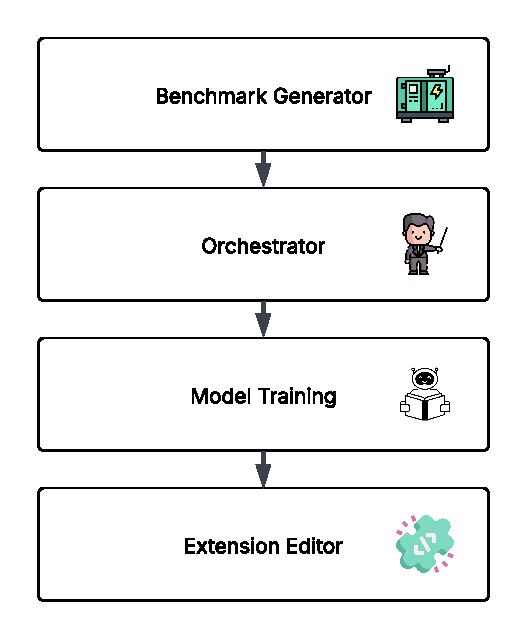
\includegraphics[scale=0.7]{figures/main_modules.pdf}
  \caption{Main modules}
  \label{fig:main_modules}
\end{figure}




In order to build the extension, it was necessary to build a system architecture capable of providing as final output the functioning tool. The architecture follows different stages, that were deeply analyzed before moving to the next one.
The architecture is divided in four main modules, Program Generator, Orchestrator, Parser, and Tool, as illustrated in Figure~\ref{fig:main_modules}.




To perform this experiment two computers were used:

\begin{table}[htbp]
\centering
\caption{System Hardware Specifications}
\begin{tabular}{|l|p{10cm}|}
\hline
\textbf{Component} & \textbf{Specification} \\
\hline
\multicolumn{2}{|l|}{\textbf{System 1 — Data Generation and Collection (High-Performance Workstation)}} \\
\hline
Operating System & Ubuntu 24.04.2 LTS (x86\_64) \\
\hline
CPU & AMD Ryzen Threadripper 3960X \\
     & 24 cores / 48 threads \\
     & Base frequency: 2.2 GHz, Boost up to ~5.05 GHz \\
\hline
Memory (RAM) & 94 GiB \\
\hline
GPU & NVIDIA GeForce RTX 3090 Ti (GA102) \\
    & VRAM: 24 GiB (standard) \\
\hline

\multicolumn{2}{|l|}{\textbf{System 2 — Machine for Testing (Lower-Spec)}} \\
\hline
Operating System & Ubuntu 24.04.2 LTS (x86\_64) \\
\hline
CPU & AMD Ryzen 5 3600 \\
     & 6 cores / 12 threads \\
     & Base frequency: 3.6 GHz, Boost up to ~4.2 GHz \\
\hline
Memory (RAM) & 16 GiB \\
\hline
GPU & NVIDIA GeForce RTX 3060 Ti \\
    & VRAM: 8 GiB (standard) \\
\hline
\end{tabular}
\label{tab:hardware_specs}
\end{table}

The more powerful system, System 1, as described in Table~\ref{tab:hardware_specs}, was used for program generation and data collection, as it was configured to work with SLURM (Simple Linux Utility for Resource Management). SLURM is a highly scalable, open-source job scheduler used to efficiently manage compute resources on shared systems. It allows tasks to be queued and scheduled based on resource availability and job priority, helping to organize workloads across users without manual intervention. The model training did not use SLURM, as it did not require significant computation time.


\section{Stage 1: Program Generator} \label{sec:work_stage1_program_generator}




To use machine learning models to predict energy consumption, it is necessary to have a large amount of data. This data can be obtained by generating programs that are then executed to collect energy profiles. The program generator is responsible for creating these programs, which are then used to train the machine learning models. The generator is designed to be flexible and adaptable, allowing it to generate a wide variety of programs based on different templates and input parameters. The architecture of the Program Generator can be seen in Figure~\ref{fig:program_generator}.


The program generator works alongside with Java Spoon to make it the more general as possible allowing custom programs to be mass generated.

The generator is capable of generating programs for custom, developer-created, Java classes, as well as for the most common APIs, such as collections interface implementations (Lists, Sets, Maps), and utility classes like Math, Base64, Duration. It can also be configured to analyze all public methods of a class or just specific ones.

\begin{figure}[htbp]%[H]
    \centering
    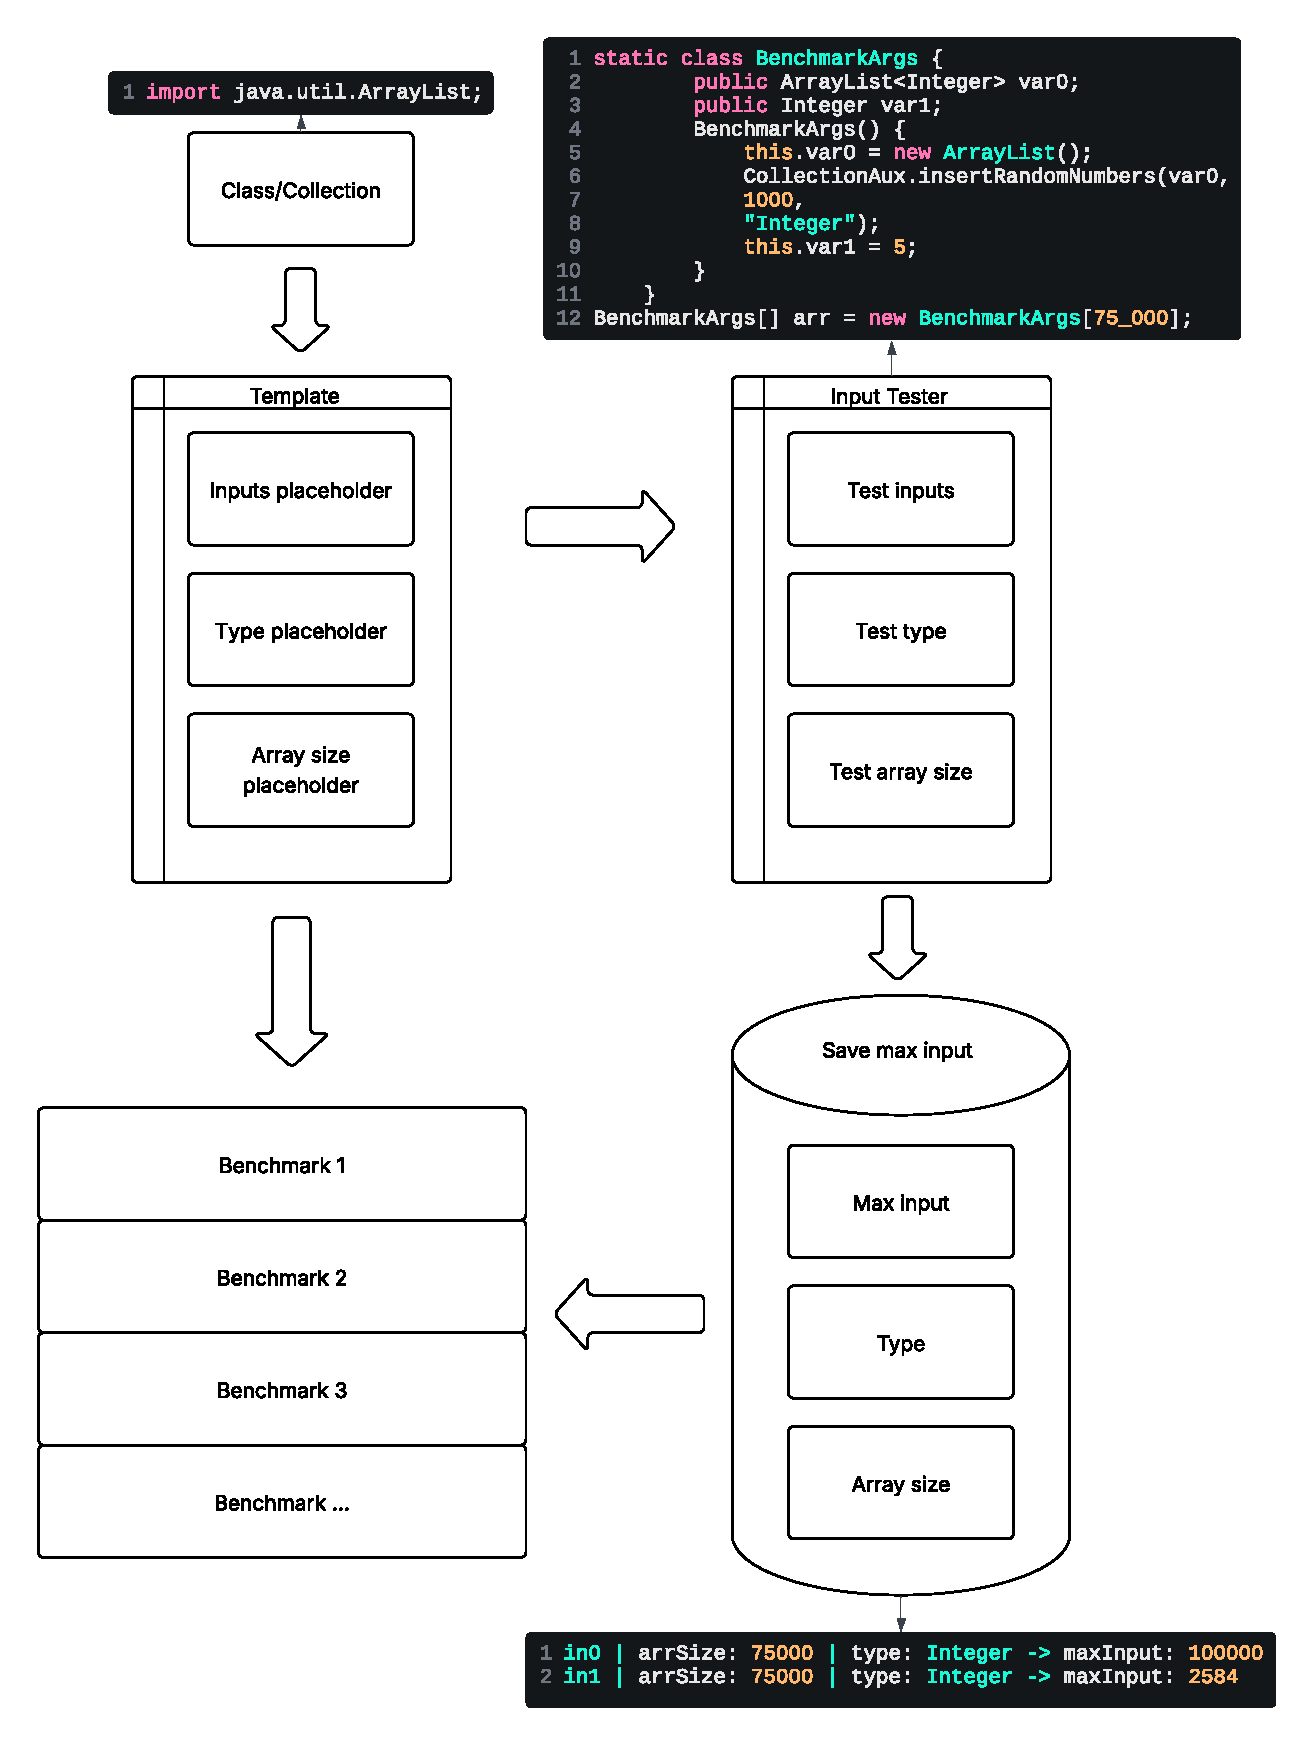
\includegraphics[width = 1 \textwidth]{figures/program_generator.pdf}
    \caption{Program Generator}
    \label{fig:program_generator}
\end{figure}


\subsection{Template Creation} \label{sec:work_stage1_template_creation}

%\FloatBarrier

%\begin{listing}[htbp]
%\begin{minted}[linenos, fontsize=\small, frame=none, bgcolor=white,breaklines=true,breakanywhere=true]{java}
%
%public class ArrayList_add_java_lang_Object_ {
%    public static void main(String[] args) throws Exception {
%        int iter = 0;
%        try {
%            BenchmarkArgs[] arr = new BenchmarkArgs["numberOfFunCalls"];
%            populateArray(arr);
%            TemplatesAux.sendStartSignalToOrchestrator(args[0]);
%            TemplatesAux.launchTimerThread(1100);
%            iter = computation(arr, arr.length);
%        } catch (OutOfMemoryError e) {
%            TemplatesAux.writeErrorInFile("ArrayList_add_java_lang_Object_", "Out of memory error caught by the program:\n" + e.getMessage());
%        } catch (Exception e) {
%            TemplatesAux.writeErrorInFile("ArrayList_add_java_lang_Object_", "Error caught by the program:\n" + e.getMessage());
%        } finally {
%            TemplatesAux.sendStopSignalToOrchestrator(args[0], iter);
%        }
%    }
%
%    static class BenchmarkArgs {
%        public ArrayList<changetypehere> var0;
%
%        public changetypehere var1;
%
%        BenchmarkArgs() {
%            this.var0 = new ArrayList();
%            CollectionAux.insertRandomNumbers(var0, "ChangeValueHere1_changetypehere", "changetypehere");
%            this.var1 = "ChangeValueHere2_changetypehere";
%        }
%    }
%
%    private static void arrayList_add_java_lang_Object_(ArrayList var, changetypehere arg0) {
%        var.add(arg0);
%    }
%
%    private static int computation(BenchmarkArgs[] args, int iter) {
%        int i = 0;
%        while (!TemplatesAux.stop && i < iter) {
%              arrayList_add_java_lang_Object_(args[i].var0, args[i].var1);
%               i++;
%        }
%        return iter;
%    }
%
%    private static void populateArray(BenchmarkArgs[] arr) {
%        for (int i = 0;i < "numberOfFunCalls";i++) {
%          arr[i] = new BenchmarkArgs();
%        };
%    }
%
%    private String input1 = "ChangeValueHere1";
%    private String input2 = "ChangeValueHere2";
%}
%
%
%\end{minted}
%\caption{Example of template for List.add(Object)}            
%\label{lst:template_example}
%\end{listing}

The first step to generate multiple programs is to first create an intermediate template capable of holding the necessary code that will later be used for energy profiling.

To generate programs for a specific class, the user has to input the name of the collection or the name of the custom program it wants to generate. For the collections of Lists, Sets and Maps, the generator is prepared to create more than one implementation of those collections, for example, if the objective is to generate programs to the List collection, the program generator will use the \texttt{ArrayList}, \texttt{LinkedList}, \texttt{Vector} and \texttt{CopyOnWriteArrayList}. The user can also input the name of the method to be analyzed, or simply gather all the available methods in the class, which are then found using Spoon.
After the search for the methods, the generator has access to all the methods it will analyze and their input parameters. Since it has access to the whole class, it can see how its constructors are called, and use them if any of the methods parameters requires. It recursively calls constructors if needed, making it very versatile to use. After identifying the methods that will be targeted, it starts by creating templates for each of them. The templates are Java classes that contain the necessary code to run the method, and placeholders for the inputs and types. The templates are structured so that they can be easily modified later, allowing the generator to create multiple programs based on the same template. The templates are designed following the structure below:

\begin{itemize}

\item Input placeholders: Placeholders that will be later changed with real values for inputs, in this case inputs are variable values. 

\item Type placeholder: Placeholders that will later be replaced with Java wrapper classes.
  
\item Array Size placeholder: Placeholder that will later be replaced with the value of an array size. (more details in~\ref{sec:work_stage2_orchestrator}). 

\end{itemize}

Also, the template is structured so that the programs will work in harmony with the \textbf{Orchestrator}, that will extract the energy profile for each program (see Section~\ref{sec:work_stage2_orchestrator}), so when the placeholders are replaced with actual values, the orchestrator can run the program, and communicate with them.


\begin{listing}[htbp]
\noindent\rule{\linewidth}{0.4pt}
\begin{minted}[linenos, fontsize=\small, frame=none, bgcolor=white,breaklines=true,breakanywhere=true]{java}
static class BenchmarkArgs {
        public ArrayList<changetypehere> var0;

        public changetypehere var1;

        BenchmarkArgs() {
            this.var0 = new ArrayList();
            CollectionAux.insertRandomNumbers(var0, "ChangeValueHere1_changetypehere", "changetypehere");
            this.var1 = "ChangeValueHere2_changetypehere";
        }
    }
\end{minted}
\noindent\rule{\linewidth}{0.4pt}
\caption{Example of variable placeholders creations}            
\label{lst:var_placeholders}
\end{listing}

Templates will have the definitions of a class that holds the necessary variables that the method under evaluation needs to run. Listing~\ref{lst:var_placeholders} shows an example of template to evaluate the method \texttt{List.add(Object)}. It follows the algorithm described in Algorithm~\ref{alg:template_creation_algorithm}. First it creates the list with the smallest constructor possible, then if the variable is a collection (List, Set, Map), or an array, it calls a custom-made method that populates collections with random values of a given type, and then it starts creating variables of parameters that the method \texttt{List.add(Object)} uses. The placeholder \texttt{ChangeValueHere1} will change to a random number, it contains a number \texttt{1} because it represents the input number of the method that will later help the model training understand how inputs can affect energy consumption. The placeholder \texttt{changetypehere} later changes to a type. The template after the transformation can be seen in the Listing~\ref{lst:var_placeholders_replaced}



\begin{algorithm}[htbp]
\caption{Template Creation Algorithm}
\label{alg:template_creation_algorithm}
\begin{algorithmic}[1]
    \Statex \textbf{Given:}
    \Statex \hspace{\algorithmicindent} $collection \coloneqq \{\text{List}\}$, collection selected.
    \Statex \hspace{\algorithmicindent} $ds \coloneqq \{\text{List, Map, Set, arrays}\}$, existent data structures.
    \Statex \hspace{\algorithmicindent} $methods \coloneqq \{\text{add, size, get}, \dots\}$, the set of methods of the classes.

    \Procedure{CreateTemplate}{}
        \State \textit{methods} $\gets$ \Call{getMethods}{\texttt{collection}}
        \ForAll{method \textbf{in} methods}
            \State vars $\gets$ empty list
            \ForAll{parameter \textbf{in} \texttt{method.parameters}}
                \State \textit{var} $\gets$ \Call{ParameterCreation}{\texttt{parameter.type}}
                \If{$parameter.type \in ds$}
                    \State \Call{FillWithRandomValues}{var, maxSizePlaceHolder, typePlaceHolder}
                \EndIf
                \State Append var to vars
            \EndFor
            \State \Call{CreateBenchmarkArrayMethod}{method, vars}
            \State \Call{CreateBenchmarkMethod}{method, vars}
            \State \Call{CreateOrchestratorStartSetup}{}
            \State \Call{CreateComputationMethod}{method, vars}
            \State \Call{CreateOrchestratorEndSetup}{}
            \State \Call{SaveTemplate}{}
        \EndFor
    \EndProcedure

    \Procedure{ParameterCreation}{\textit{type}}
        \If{\Call{IsPrimitive}{type}}
            \State \Return type
        \Else
            \State dependencies $\gets$ \Call{GetConstructorArguments}{type}
            \State args $\gets$ empty list
            \ForAll{dep \textbf{in} dependencies}
                \State arg $\gets$ \Call{ParameterCreation}{dep}
                \State Append arg to args
            \EndFor
            \State instance $\gets$ \Call{Instantiate}{type, args} \Comment{Create an instance, using the smallest constructor.}
            \State \Return instance
        \EndIf
    \EndProcedure
\end{algorithmic}
\end{algorithm}



\begin{listing}[htbp]
\noindent\rule{\linewidth}{0.4pt}
\begin{minted}[linenos, fontsize=\small, frame=none, bgcolor=white,breaklines=true,breakanywhere=true]{java}
static class BenchmarkArgs {
        public ArrayList<Integer> var0;

        public Integer var1;

        BenchmarkArgs() {
            this.var0 = new ArrayList();
            CollectionAux.insertRandomNumbers(var0, 1000, "Integer");
            this.var1 = 10;
        }
    }
\end{minted}
\noindent\rule{\linewidth}{0.4pt}
\caption{Example of variable placeholders replaced}            
\label{lst:var_placeholders_replaced}
\end{listing}



It is worth mentioning that the types used by the generator are the Java wrapper classes, which are object representations of the primitive types. Using these types it is possible to achieve a more general generator, as every program can use them and if other custom types were used it would make the generator more complex and not general.

What mostly differs from template to template is the number of variables used, because different methods have different parameters, so the template can have more or less input placeholders, also the type placeholder changes according to the methods types and parameters.


Creating the template for each method allows cutting off time of the program generation by only having to replace values of the placeholders instead of needing to create the whole program all over again, since the programs for the same method only differ in inputs, types and array size, maintaining all the structure.

\subsection{Input Tester} \label{sec:work_stage1_input_tester}

An important aspect of the program generator are the inputs it generates. Every method has its on funcionality that may be dependent on the input values.  To be able to better generalize, it is important to find the method input values upper limit. Knowing the maximum size that different parameters can have is fundamental as it needs to be representative, so the energy profiles can cover more cases, but not to large so that the programs start to get out of memory or taking too much time to complete.
The limit definition works by using binary search. It has an inital threshold on the inputs (e.g., 1-100,000 to numerical values) and it starts by trying to run the program with the half of the maximum upper limit threshold (e.g., 50,000). 

It can be important, for pratical reasons, to impose a threashold on the execution time (in this project, we established the threshold as 10 seconds based on empirical experimentation). If the program runs successfully, it will increase the input by half, and if it fails, it will decrease the input by half. This process continues until the maximum value for the input is found.

If the method that is being tested has more than one input, the input tester is responsible to find the upper limit for each parameter individually. First it sets all the input values to 1 and then starts the binary search individually for each of the parameters one by one while leaving the other parameters with the value of 1. Although this is a simplification, this method avoids having to find multiple combinations of parameters which would increase the time complexity exponentially. More robust solutions (such as using a combinatory search) could be implemented in the future. Nevertheless, even using the simplified solution, the process of finding the max inputs is time-consuming. To improve its performance, when the maximum value is found, the values of the input type, maximum value and order (e.g., first, second or third parameter), are stored in a file. This makes subsequent executions much faster. It is worthy to mention that the maximum inputs found depend heavily on the machine where the program generation is taking place, as different hardware will change the maximum values allowed for the inputs. Example 1 illustrates how the input tester works for the method \texttt{List.add(index, Element)}.

\begin{tcolorbox}[
    title=Example 1: Input Testing Process for \texttt{List.add(index, Element)},
    colback=gray!5!white,
    colframe=gray!75!black,
    fonttitle=\bfseries,
    breakable,
    label={box:add-method-testing}
]

Consider analyzing the \texttt{add} method of a list with the following parameters:
\begin{itemize}
    \item \texttt{arg0}: Size of the list (integer)
    \item \texttt{arg1}: Index at which to insert the new value (integer)
    \item \texttt{arg2}: Value to be added (integer)
\end{itemize}

\textbf{Step 1 – Varying \texttt{arg0} (list size):}

\begin{itemize}
    \item Iteration 1: \texttt{arg0 = 25,000}, \texttt{arg1 = 1}, \texttt{arg2 = 1}
    \item Iteration 2: \texttt{arg0 = 12,500}, \texttt{arg1 = 1}, \texttt{arg2 = 1}
    \item Iteration 3: \texttt{arg0 = 6,250}, \texttt{arg1 = 1}, \texttt{arg2 = 1}
    \item $\vdots$
    \item Final Iteration: \texttt{arg0 = 1,700}, \texttt{arg1 = 1}, \texttt{arg2 = 1}
\end{itemize}

\textbf{Step 2 – Varying \texttt{arg1} (index):}

\begin{itemize}
    \item Iteration 1: \texttt{arg0 = 1}, \texttt{arg1 = 25,000}, \texttt{arg2 = 1}
    \item Iteration 2: \texttt{arg0 = 1}, \texttt{arg1 = 12,500}, \texttt{arg2 = 1}
    \item $\vdots$
    \item Final Iteration: \texttt{arg0 = 1}, \texttt{arg1 = 1}, \texttt{arg2 = 1}
\end{itemize}

{Note: Since the list size (\texttt{arg0}) remains 1, the maximum valid index (\texttt{arg1}) is constrained to 1. This reveals a limitation in the input testing approach.}

\textbf{Step 3 – Varying \texttt{arg2} (value to be added):}

\begin{itemize}
    \item Iteration 1: \texttt{arg0 = 1}, \texttt{arg1 = 1}, \texttt{arg2 = 25,000}
    \item Iteration 2: \texttt{arg0 = 1}, \texttt{arg1 = 1}, \texttt{arg2 = 37,500}
    \item $\vdots$
    \item Final Iteration: \texttt{arg0 = 1}, \texttt{arg1 = 1}, \texttt{arg2 = 100,000}
\end{itemize}

\textbf{Final stored input limits:}
\begin{itemize}
    \item \texttt{arg0} — \texttt{integer} — \texttt{1,700}
    \item \texttt{arg1} — \texttt{integer} — \texttt{1}
    \item \texttt{arg2} — \texttt{integer} — \texttt{100,000}
\end{itemize}

\end{tcolorbox}


The fact that the input has a pre-determined range it allows using binary search which makes the search much faster than linear search.
Nevertheless, the input search does not come without some limitations. First it is constrained to identifying valid input values within the range. As an example, throughout this project we dealt frequently with lists and collections, which require a minimum size of 1 to function correctly. Although this value can be changed in the future, for now it ensures compatibility with most common data structures. The higher bound was chosen due to empirical evidences, as larger input values would lead to limitating execution times and memory crashes. Another constraint is on how the input handles multiple parameter methods. During its search for a valid input, it needs to fix all the other parameters that is not searching, with a default value (typically the lower bound). This approach simplifies the testing process and improves efficiency by avoiding the exponential complexity of testing all possible parameter combinations. However, it will introduce limitations in cases where the parameters are interdependent, which can lead to not estimating the real highest input possible. 
Despite these limitations, the input search plays a crucial role in ensuring that the program generator produces viable test cases. By identifying input ranges that are both valid and computationally achievable, it reduces the unusable generated programs (e.g., due to timeouts or crashes), and maximizing the number of generated programs, that can be used for energy profiling.



\subsection{Program Generation} \label{sec:work_stage1_program_generation}

Finally, when the templates are created, and the maximum inputs are found the program generation can finally begin. This part consists on picking every template created and replacing the placeholder values with actual values created by a random number generator. It follows the algorithm described in Algorithm~\ref{alg:template_fullfillment_algorithm}

It starts by looping through the types and changing them to the Java wrapper classes, then it loops through the array size. Lastly, it loops through the input sizes determined by the input tester and can repeat this process a configurable number of times. By increasing the number of iterations, results in more programs being generated with random inputs, constrained by the previously identified input bounds. 




\begin{algorithm}[htbp]
\caption{Template Fullfillment Algorithm}
\label{alg:template_fullfillment_algorithm}
\begin{algorithmic}[1]
    \Statex \textbf{Given:}
    \Statex \hspace{\algorithmicindent} $templates$, list of templates previously generated.
    \Statex \hspace{\algorithmicindent} $types \coloneqq \{\text{Integer, Double, Long, Float, Short, Character }\}$, types to be replaced.
    \Statex \hspace{\algorithmicindent} $arraySize \coloneqq \{\text{75\,000, 100\,000, 150\,000}\}$, array sizes to be used.
    \Statex \hspace{\algorithmicindent} $template.maxInputs $, each template has a maximum input file associated to it.
    \Statex \hspace{\algorithmicindent} $iterations $, number of iterations for the input loop.

\Procedure{FullfillTemplate}{}
    \ForAll{template \textbf{in} templates}
        \ForAll{type \textbf{in} \texttt{types}}
            \State program $\gets$ \Call{Replace}{template, "typePlaceHolder", type}
                \ForAll{arraySize \textbf{in} \texttt{arraySizes}}
                    \State program2 $\gets$ \Call{Replace}{program, "arraySizePlaceHolder", arraySize}
                        \For{$i \gets 0$ \textbf{to} \texttt{iterations}}
                            \State program3 $\gets$ \Call{replaceValues}{program2, template.maxInputs}
                            \State \Call{SaveToFile}{program3}
                        \EndFor
                \EndFor
        \EndFor
    \EndFor
    
\EndProcedure

\vspace{1em} 

\Procedure{ReplaceValues}{program, maxInputs}
    \State valuesToReplace $\gets$ \Call{FindStringsToReplace}{program, placeholderPattern}
    \For{$i \gets 0$ \textbf{to} \Call{Size}{valuesToReplace} - 1}
        \State value $\gets$ valuesToReplace[i]
        \State type $\gets$ \Call{ExtractType}{value}
        \State max $\gets$ maxInputs[i]
        \State min $\gets$ \Call{Min}{1, max}
        \State newValue $\gets$ \Call{GetRandomValue}{type, min, max}
        \State program $\gets$ \Call{Replace}{program, value, newValue}
    \EndFor
    \State \Return program
\EndProcedure

\end{algorithmic}
\end{algorithm}

This process easily generate thousands of programs which are crucial to train machine learn models that are able to predict energy consumption. When generating programs, a number is chosen to balance the requirements for effective model training while minimizing the time spent on input testing and collecting energy profiles. Afterwards, that the programs are ready to be compiled and used.



\section{Stage 2: Orchestrator} \label{sec:work_stage2_orchestrator}




Having all the programs generated, it is possible to move to the next stage. Gathering the energy profiles for each of the generated programs. 
Energy profiles~\cite{10.1145/2884781.2884869,8816747} are an established way to organize energy consumption data. They will be the main data source of the machine learning models to obtain accurate results. To reduce the complexity of this task, a process was implemented, illustrated in Figure~\ref{fig:orchestrators_workflow}. This process automates the task while taking into account what was mentioned in Section~\ref{sec:background_benchmarking}.

As described in the Section~\ref{sec:background_energy} there are several tools capable of performing dynamic energy measurements.

PowerJoular has good features that caught our attention, for example being a command line tool that could be easily integrated in almost every programming language, it stores the energy used in a CSV file, capable of only reading energy of running processes and so on, as explained before in Section~\ref{sec:background_energy}.

Since PowerJoular is a command line tool, it is launched as a process, and then it can be killed whenever needed because it is a process as well. This allows to measure not only programs/processes energies but have a more precise measurement, as it is possible to call PowerJoular to measure a specific computation and then kill it when the computation is finished.

With all of this in mind a process was built. The process uses an orchestrator that is responsible for invoking the target program and the measurement tool (PowerJoular) to accurately measure the energy consumption of the program or the specific computation being analyzed within it.


One challenge in measuring energy consumption is that computation often completes too quickly to capture accurately. It is hard to measure a single operation of, for example, a \texttt{List.\allowbreak add(Object)} with most tools, as it simply to fast for the tool to capture, and if the tool was able to capture it, the energy measured could have too much noise to be considered. Our solution was to loop through the method until the tool is capable of getting its energy and then dividing the total energy by the number of times it looped. 
This solution, although effective, introduces potential errors that need to be addressed.

By approaching the measurements with the loop technique, first we need to create the variables needed for the method target to analysis, like shown in the Listing~\ref{lst:var_placeholders} \wo{dê exemplos}. However, because, the methods are treated like a black box, it is not possible to know what the methods are going to do with the parameters or with its variables. {\color{blue} For example, the method \texttt{List.size()} has no parameteres, and return the size of the list. In this case the functioning of the method is known, and it is noticeable that the attributes of the object will not change, as the method simply reads and returns a value.

However, this raises problems with other methods, such as \texttt{List.add(Object)}. This method will insert values in the list, increasing its size. This increase in size can lead to different behavior of the method as the internal object changes in each iteration. In this case, inserting into a smaller list can produce different measurements of inserting into a larger list.}

Now, suppose we have a method called \texttt{sort} that takes a randomly ordered list and sorts it. This introduces a problem when measuring its energy consumption. On the first run, the method will sort the unsorted list, which may take significant time depending on the randomness of the data and the sorting algorithm used. However, on subsequent runs with the same list, the input is already sorted, meaning the sort method will likely complete much faster or with minimal effort. This difference can result in misleading or inconsistent measurements.

To prevent this side effect from happening we designed a solution that consists of creating an array that holds the parameters, that can be seen in the Figure~\ref{fig:array}. The necessary parameters to execute the method are created and stored into the array. They are exactly copies with different refereces. Now, if one of the elements is changed during its execution on the method, it will not affect the other's execution. Since this approach increases memory usage due to multiple copies, we empirically selected array sizes (75,000, 100,000, and 150,000) to balance between avoiding out-of-memory errors and ensuring the computation runs long enough for PowerJoular to record energy measurements. PowerJoular by default needs to run for 1 second to create the CSV file that has the energy used for the target process, so these sizes aim so that looping the array takes at least a second. In some cases, the CSV file may not be generated because the loop executes too quickly. In such instances, the energy reading will be assumed to be 0 J, as the execution was too fast to record a value.


\begin{figure}[htbp]
  \centering
  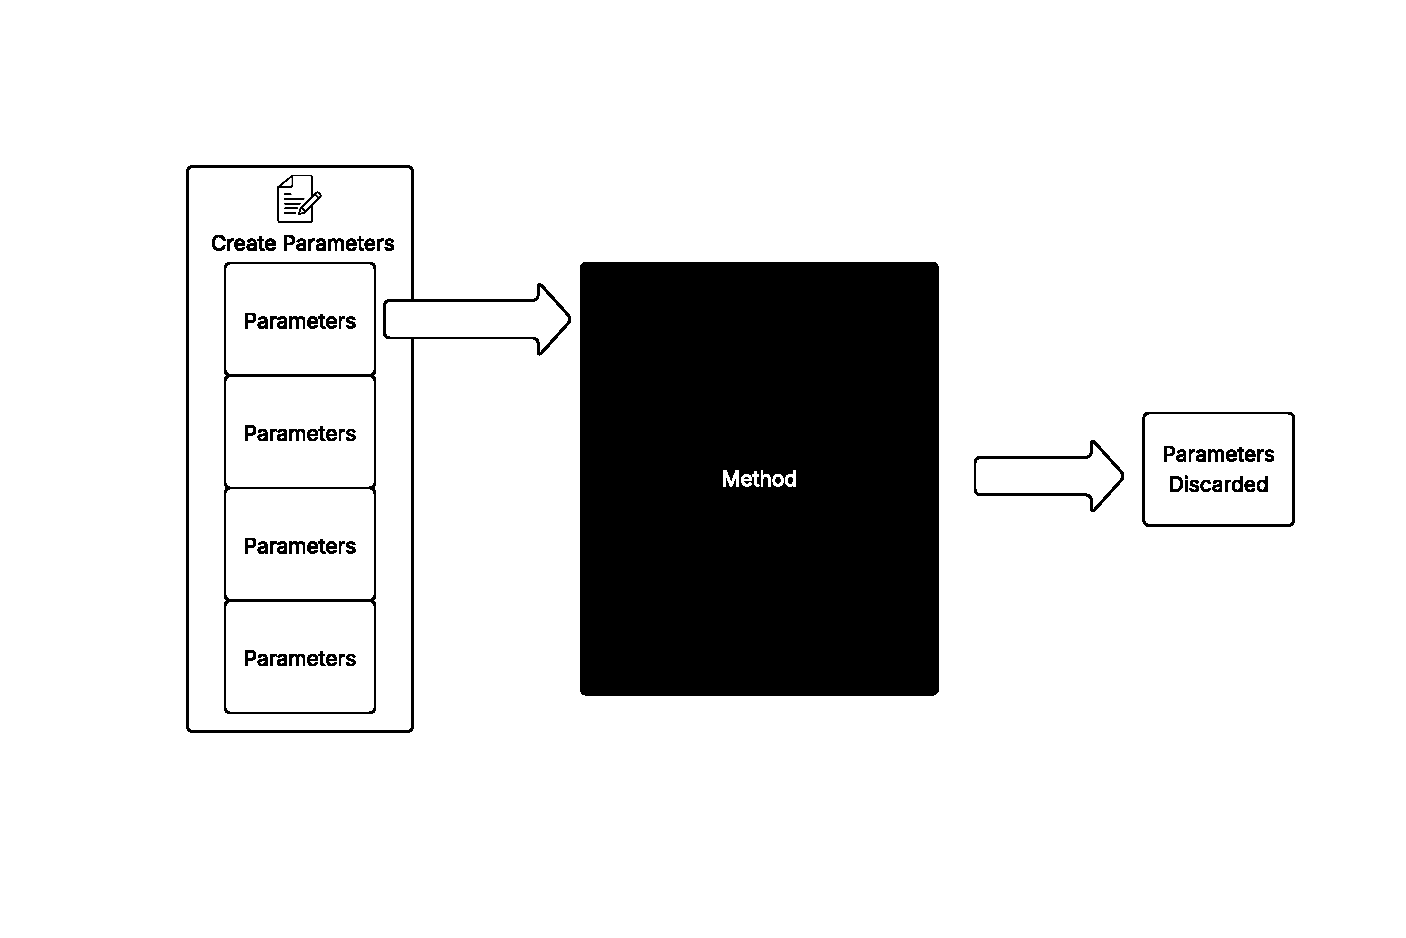
\includegraphics[width = 1 \textwidth]{figures/array.pdf}
  \caption{Array example}
  \label{fig:array}
\end{figure}

To be able to collect some faster executions, the original PowerJoular was modified to allow customizable measurement durations, enabling readings at intervals shorter than the default 1 second, such as 100ms, which provides greater flexibility and finer granularity in energy profiling.

The computation method shown in Listing~\ref{lst:Computation_method} illustrates how each profiling method operates independently of the specific method being evaluated. It attempts to execute the target function repeatedly for approximately one second. In this particular case, the target function performs the operation \texttt{var.add(arg0);} and returns the number of iterations completed, which is then used for further calculations.

\begin{listing}[htbp]%[H]
\noindent\rule{\linewidth}{0.4pt}
\begin{minted}[linenos, fontsize=\small, frame=none, bgcolor=white,breaklines=true,breakanywhere=true]{java}
private static int computation(BenchmarkArgs[] args, int iter) {
        int i = 0;
        while (!TemplatesAux.stop && i < iter) {
              arrayList_add_java_lang_Object_(args[i].var0, args[i].var1);
               i++;
        }
        return iter;
    }
\end{minted}
\noindent\rule{\linewidth}{0.4pt}
\caption{Computation method}            
\label{lst:Computation_method}
\end{listing}


With the process structure now defined, we can proceed to explain how it functions.

The workflow of this step can be described as follows:


\begin{figure}[htbp]
  \centering
  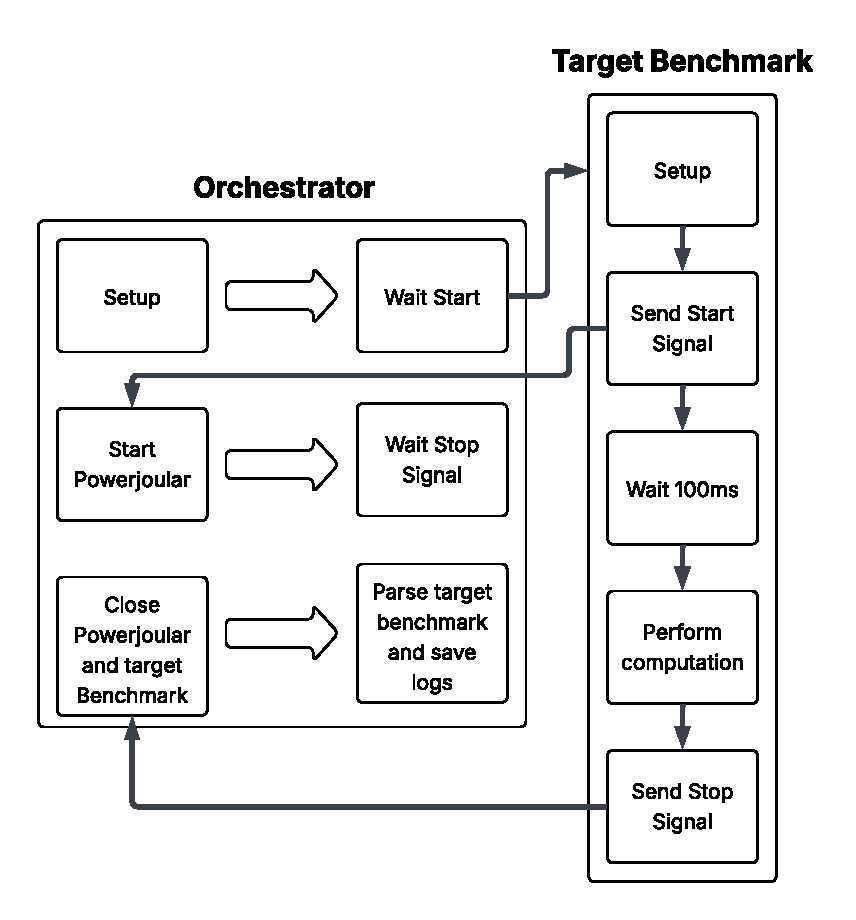
\includegraphics[scale = 0.7]{figures/orchestrators_process.pdf}
  \caption{Orchestrator Workflow}
  \label{fig:orchestrators_workflow}
\end{figure}

\begin{itemize}
  \item The orchestrator launches a command to start the target Java Program and waits a signal.
  \item The Java program starts and setup the necessary elements to run (creating all the variables, reading/writing files, populating the array, etc.) and then before starting the computation it wants to measure, it sends a start signal to the orchestrator to start monitoring, and waits for 100 milliseconds.
  \item The orchestrator receives the start signal and reads the PID, which is stored in a file during the target program setup. Finally, it starts PowerJoular using that PID. Then it waits for the stop signal.
  \item The Java program will run until it finishes the computation. The computation runs for a maximum of one second. Then the number of iterations are stored in a file and the stop signal is sent back to the orchestrator.
  \item The orchestrator on receiving the stop signal, first stops PowerJoular and then stops the target program, if needed. Then it parses the target program to extract its features, combines them with the energy information stored in the files created by PowerJoular, stores it in a CSV file.
\end{itemize}

All these steps are performed for each generated program. At the end of the process, a log file is created containing key information, including all the programs used, the PowerJoular files generated, temporary files, error logs, and features.


\section{Stage 3: Model Training} \label{sec:work_stage3_model_training}

Now, that all the energy profiles are collected it is possible to finally start training the models. As explained in \ref{sec:background_machine_learning} there are a lot of possible ways of using machine learning, however in this case the approach that best fit our need is supervised machine learning. So, some models were trained to see how good they performed using the data collected.

First there is a merge of features. While each method is initially trained individually, it is not useful to treat LinkedList.add(Object) and ArrayList.add(Object) as entirely separate cases. Both represent the same List.add(Object) method, differing only in their characteristics specific to their implementation. Therefore, once all energy profiles have been collected, a merging step is performed to consolidate these related methods.

All these features are stored in a new CSV and for the python program in a Data frame, to be processed.

This part was developed in python using some libraries specialized on machine learning, like scikit-learn (sklearn)~\cite{scikit-learn} which contains some models and functions to evaluate the models, and PySR~\cite{cranmer2023interpretablemachinelearningscience} which was already explained in \ref{sec:background_machine_learning} an is also already implemented.

In this phase the models tested were: Decision Tree Regressor, Random Forest, Gradient Boosting, Linear Regression, and PySR.

First the values of the MSE and R2 are evaluated by the default values of sklearn, then in a second pass, GridSearch was used, which is a function of sklearn that tries to find the best parameters for a model. After that the scores and models are saved. The GridSearch does not work with PySR as they are from different libraries so, the parameters for PySR were manually set.

In the end the chosen model was PySR as it can represent the predictions in expressions which can help the users to try to understand why the code is using more energy. It has a nice feature of allowing to balance complexity and accuracy. And can easily be used in another code language as it is represented as a mathematical expression.



\section{Stage 4: Extension Build} \label{sec:work_stage4_extension_build}

The last stage was to build an extension for an IDE, VSCode. This extension allows the user to have a better understanding of how much energy the code is consuming, and what are the methods, and variables that most affect it.
When opening the extension side page, it contains some sliders that can change the input values, and it has the estimate button, to predict the energy.
The sliders are updated when the document is saved.%, rather than on every change, to prevent performance slowdowns.

The extension works by parsing the Java file of the user, and gathering all the methods used that are already models that are trained. Then it finds which variables affect those methods, meaning the variables that are the inputs to the method, for example, in \texttt{list.add(i);}  the inputs and important variables are \texttt{list} and \texttt{i}.
The extension does this to every method it finds and groups it by method. In the end it creates groups of input variables for each method, and displays it in sliders. The sliders allow the user to change the input values and when pressing the estimate button, depending on the changed values, it will change the energy estimation.

If a method calls another user-defined method that already has an assigned energy cost (but is not a trained method), then the calling method will also include that energy cost.

When a trained method is called inside a loop, a new slider appears to represent the loop size. The method’s energy cost is multiplied by this loop size. In the case of nested loops, the energy cost is multiplied by the product of all nested loop sizes.

Note that only methods and variables that affect the energy appear on the panel.






%\section{Step 3: Implementation and testing} \label{sec:work_step3_implementation_and_testing}
%
%Once the main components of the tool are built, they need to be assembled into the extension. When using it, the developers should be able to see the total energy estimate of their code in the IDE, and it should also show the estimates for each function and its most energy consuming lines.
%The estimate alone may be enough to understand if the code is high or low in energy consumption, for example, if the developer has two implementations of the same function and they both give different values, it may be easy to understand which one consumes the most. However, this may not always be the case, so the tool will also provide some information to help the developer know how good or bad the energy efficiency of the code is.
%
%Another important step is to test and ensure that the tool performs as expected on most machines, delivers the most accurate estimations possible, and undergoes a final comparison with other tools to evaluate its effectiveness.
%